\chapter{Computer Modelling and the Forward Problem}

\section{Problem Statement}

The goal is to obtain measurements of energetic electron precipitation spectra and fluxes. Direct measurements of the electrons are not always practical, except for instrumented sounding rockets, since the  precipitating electrons deposit their energy in a region of the atmosphere (approximately 80 to 100 kilometers) that is difficult to reach for durations longer than a few minutes~\citep{Berger1972}. Satellites in low Earth orbit can accomplish measurements of precipitation, but only along their relatively short passes through the region of interest. 

The X-ray photons emitted by the precipitating electrons as they decelerate penetrate deeply into the atmosphere and are detectable at altitudes above approximately 30 kilometers from the ground. This region of the atmosphere is accessible by stratospheric balloons, capable of flights which can extend for days or weeks, which makes them an attractive platform for longer term measurements. In this chapter, a model is created which predicts the photon measurements a high altitude balloon would observe for a given electron precipitation event. 

This is not a new problem, measurements of X-ray spectra from high altitude balloons have an extensive heritage. The purpose of this chapter is to review the models which already exist and then to develop a similar model, tailored to the instrumentation discussed in Chapter 3. There will be an emphasis on computation speed, so that the model can be evaluated over large parameter spaces quickly on ordinary hardware. This will be particularly important when the inverse problem - attempting to reconstruct electron spectra from X-ray measurements - is attempted in Chapter 5. Additionally, the model we create will be designed to separate dependent variables as much as possible, so that it can be applied to different experiments and different instruments with few modifications. 

\section{Scattering and Energy Deposition Physics}

For the problem at hand, classical physics (with relativistic effects) offers a sufficient description of the energy deposition and radiation caused by electrons as they travel through the atmosphere. Electrons from space enter the upper atmosphere at relativistic energies, ranging from less than 100 keV to several MeV. As the electrons penetrate the atmosphere, they interact with the neutral constituents of the atmosphere. These interactions are elastic and inelastic scattering.

Elastic (Rutherford) scattering was discovered through an experiment consisting of a  beam of alpha particles incident on a sheet of thin gold foil. This lead to the discovery of the atomic nucleus by observing that few alpha particles were deflected, and when this happened, they were mostly deflected through large angles, implying that most of the atomic mass was concentrated in a small region in the centre of each atom. In this interaction, neither the nucleus or the scattered alpha particle is excited or changes state, implying that both kinetic energy and momentum are conserved. For electrons scattering from nuclei at keV to MeV energies, relativistic effects need to be taken into account. The name Mott scattering is used in this case. 

When inelastic scattering occurs between an electron and an atomic nucleus, kinetic energy which is lost by the electron is emitted as a photon. The term used for this process is Bremsstrahlung, a german word for the term ``braking radiation''. The Larmor formula, and its relativistic generalization are the well-known descriptors of the radiation emitted by this process. The power radiated by an accelerating charged particle is given classically as:

$$P = \frac{2}{3}\frac{q^2}{m^2c^3}\lvert \mathbf{\dot{p}} \rvert^2$$

where q is the particle charge, m is its mass, and $\mathbf{\dot{p}}$ is the time derivative of its momentum. The relativistic generalization of this formula is:

$$P = \frac{2 q^2 \gamma^6}{3c} \left( \dot{\mathbf{\beta}}^2.- (\mathbf{\beta}\times\mathbf{\dot{\mathbf{\beta}}}^2)\right)$$

where $\beta$ is the velocity as a fraction of the speed of light, $v/c$ and $\gamma$ is the relativistic factor. There are also expressions for the angular distribution of the radiated power. 

Interaction probabilities for electron scattering are a function of energy, and are characterized by a quantity called the cross section. The definition is constructed by considering a particle incident on a target, which is scattered through an angle $\theta$. Define the impact parameter $b$ as the distance of closest approach to the target. Define the area element $d\sigma = b d\phi db$, in the plane of the impact parameter. The differential cross section is the ratio $\frac{d\sigma}{d\Omega}$, where $d\Omega$ is the differential solid angle through which the incident particle is scattered. 

Cross sections can be experimentally measured, and also derived from theory. For Bremsstrahlung photons emitted by inelastic scattering from atomic nuclei, the electron cloud of the atom complicates the resulting expressions. Usually the process is complex enough that specific assumptions need to be made for derivations which apply in different energy ranges. For the problem of Bremsstrahlung emission by energetic electrons in the atmosphere, there is a synthesis of theoretical and experimental measurements which can be used to obtain electron energy loss as a function of depth in the atmosphere~ \citep{Berger1972}. Once a Bremsstrahlung photon is produced, it then propagates through the atmosphere and undergoes its own interactions. Photoelectric absorption, multiple scattering, and Compton scattering all have to be taken into account to predict the paths that photons will take in the atmosphere~\citep{Berger1972}. This complicates the analysis of the causative electron spectrum significantly. In the photoelectric process, a photon impacts a neutral atom and causes an electron to be emitted. This process is dominant at lower energies (less than 511 keV approximately), beyond which Compton scattering becomes more relevant. Compton scattering is inelastic scattering between a photon and electron, which results in a longer wavelength photon and a recoiling electron. Finally, at energies beyond 1.022 MeV, pair production can occur where a photon is converted into an electron positron pair. The pair subsequently annihilates, releasing a pair of photons. 

\section{Previous results on Energetic Electron Precipitation}

Approximations and descriptions of electron precipitation, the resulting production of X-ray photons, and their subsequent transport through the atmosphere have existed for a long time. An early comprehensive review was carried out by~\citet{Brown1966a}. The first approximations of this processes ignored multiple scattering (\citet{Anderson1960}, \citet{Brown1965}, \citet{Christensen1970}, \citet{Barcus1966}, \citet{KAMIYAMA1966}, \citet{Polk1965}). The first attempt with the effects of multiple scattering included was done by~\citet{Rees1963}. The method used was based on empirical measurements of the energy dissipation of electrons in air.

There are some findings from ~\cite{Rees1963} which can be used to make our analysis of the problem more simple. They note that the effect of the Earth's magnetic field, which can roughly be thought of guiding incident electrons, shouldn't have a significant effect on the energy deposition altitude profiles. This is a big simplification, because the Monte Carlo simulations we will employ are highly sensitive to the simulation spatial scale. Ignoring the effects of the magnetic field allows effects which occur on the scale of the electron gyrofrequency to be ignored, making the simulations much faster. As noted by ~\cite{Berger1972}, the number of photons which survive to detection is small compared to the number of incident electrons. This implies that Monte Carlo simulations of the resulting photon spectra will be expensive, so to obtain statistically meaningful results, simulation speed is important. 

Another important result from ~\cite{Rees1963} is that the initial angular distribution of the precipitating electrons has only a minor effect on the energy deposition profiles, once the total path length through the atmosphere is accounted for. This has two implications: on one hand, the problem of finding X-ray photon spectra corresponding to precipitating electron spectra becomes a single dimensional problem in energy, rather than a two dimensional one in angle and energy. This represents a large simplification. On the other hand, this also implies that obtaining information about the angular distribution of the precipitating electrons from X-ray measurements is a difficult problem. Our approach in this chapter will be to verify this fact through simulation, and then apply the problems insensitivity to electron angular distribution as a useful simplifying assumption. 

~\cite{Berger1972} provide the number of X-ray photons created per incident electron as a function of electron and X-ray energy, for a given altitude in the atmosphere. These curves are reproduced in Figures~\ref{berger_seltzer_curves_0},~\ref{berger_seltzer_curves_1}},~\ref{berger_seltzer_curves_2}} for altitudes of 32, 34, and 40 kilometers above ground. The strong dependence on the photon population to the sample altitude is apparent, as well as the characteristic shape of the photon spectra. Their results show that one aspect of the problem that cannot be ignored is the dependence on detector altitude. For a given experiment, this will need to be recorded, and the model run at the same altitude. 

It is prudent to again emphasize at this point that modelling the production of X-rays in the atmosphere caused by precipitating electrons is not a new problem. We need to make a model similar to those of ~\cite{Rees1963} and ~\cite{Berger1972}, not because their results are incorrect, but because we need the flexibility of repeated model runs under different scenarios. Further, when the inverse problem of determining causative electron spectra based on X-ray measurements is attempted in the next chapter, the energy resolution needed in the model output will exceed that of the data provided by these authors.

In~\cite{Berger1972}, resultant X-ray spectra are shown which correspond to mono-energetic beams of electrons. This can be thought of as a Green's function approach to the modelling problem. Evaluating the model for every input electron spectrum of interest is not necessary, provided that the mapping between the input and output is linear. Since the state of the atmosphere is not altered significantly by incident beams of precipitating electrons, different electron beams will produce X-ray spectra which combine additively. For the same reason, the intensity of the resulting X-ray beam will scale linearly with the intensity of the beam of precipitating electrons. In the Green's function approach, beams of mono-energetic electrons are modelled, and the resulting X-ray energy spectra are used to form the columns of a matrix. This matrix then maps between electron energy spectra and X-ray energy spectra for a given altitude. Provided the angular distribution of the incoming electrons can be neglected, and the responses to individual mono-energetic beams can be evaluated to sufficient statistical purity, then model runs for arbitrary precipitating electron spectra can be produced with a single matrix multiplication. 

\begin{figure}[p]
\label{berger_seltzer_curves_0}
\centering
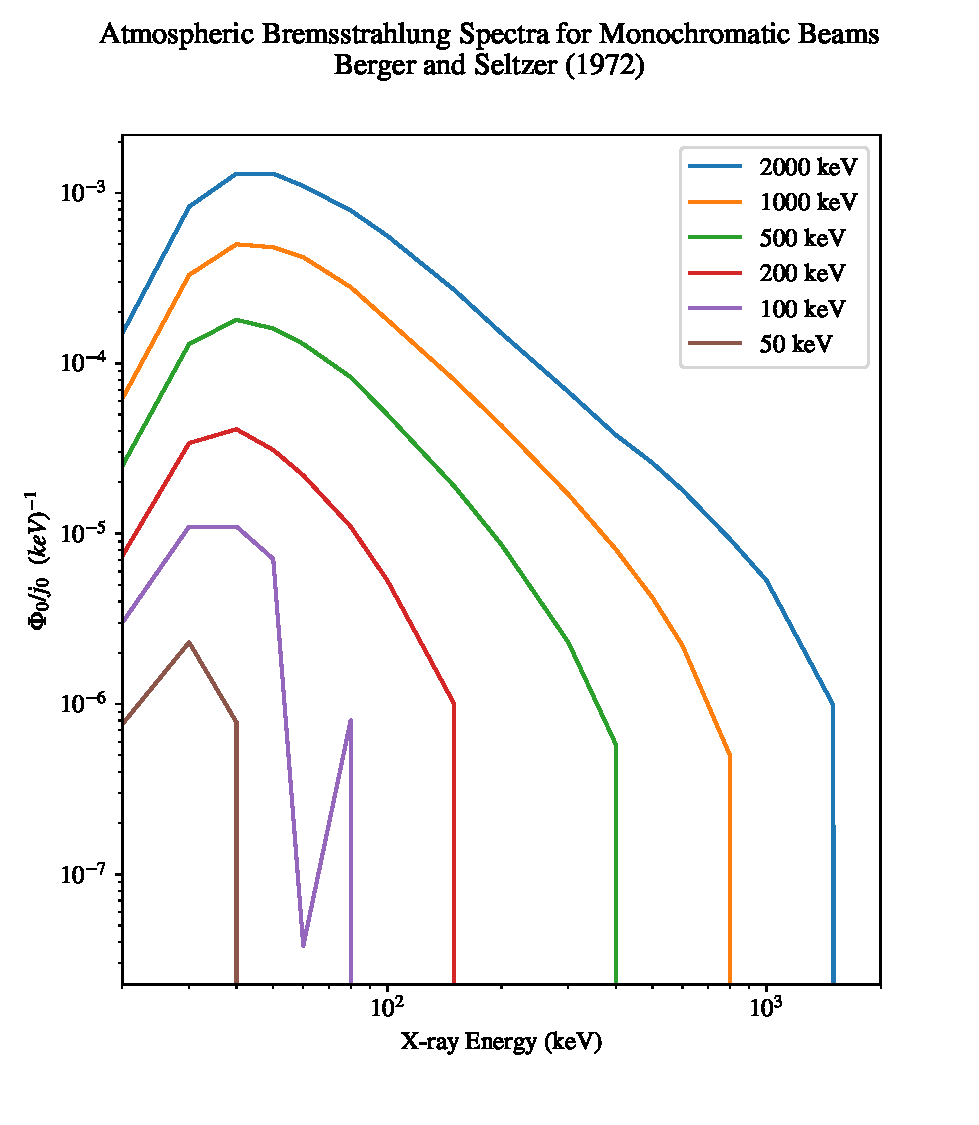
\includegraphics[width=1.0\textwidth]{figures/chapter_3/berger-seltzer-curves/berger_seltzer_curves_0}
\caption{X-ray photon flux per incident electron flux for different incident electron beam energies, from ~\cite{Berger1972} for an altitude of 32 km.}
\end{figure}

\begin{figure}[p]
\label{berger_seltzer_curves_1}
\centering
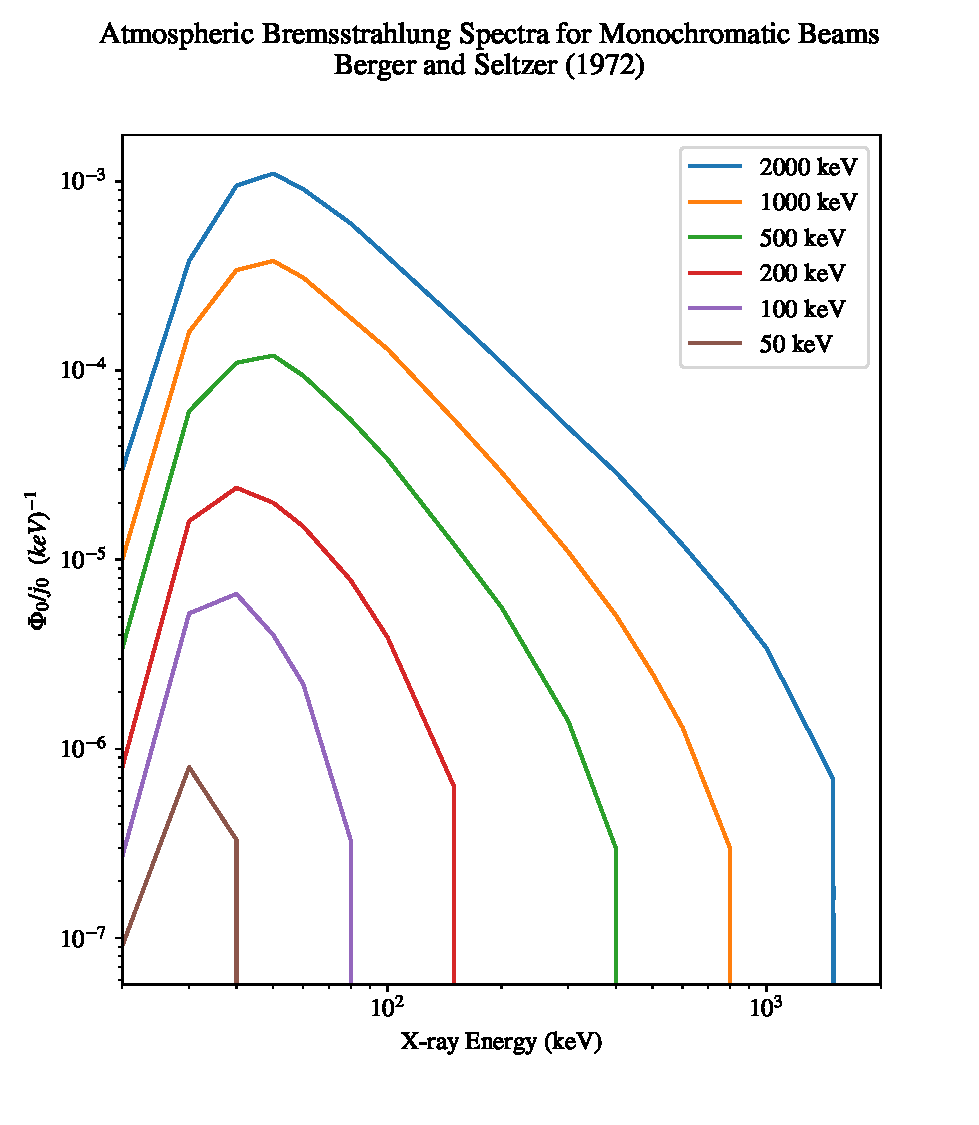
\includegraphics[width=1.0\textwidth]{figures/chapter_3/berger-seltzer-curves/berger_seltzer_curves_1}
\caption{X-ray photon flux per incident electron flux for different incident electron beam energies, from ~\cite{Berger1972} for an altitude of 34 km. }
\end{figure}

\begin{figure}[p]
\label{berger_seltzer_curves_2}
\centering
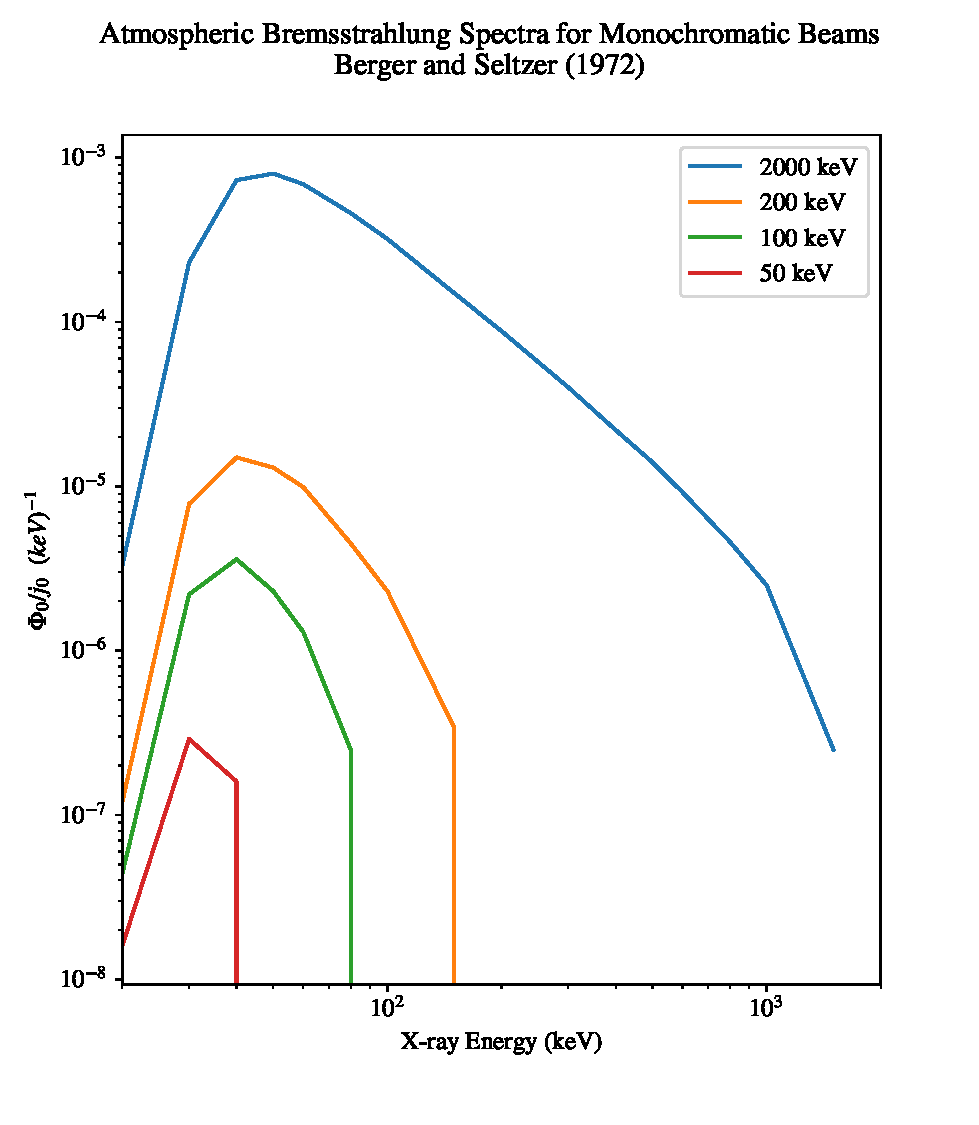
\includegraphics[width=1.0\textwidth]{figures/chapter_3/berger-seltzer-curves/berger_seltzer_curves_3}
\caption{X-ray photon flux per incident electron flux for different incident electron beam energies, from ~\cite{Berger1972} for an altitude of 40 km. }
\end{figure}

\section{GEANT4 and Monte Carlo Simulations}

There are several computer software packages used to simulate the transport of radiation through matter. Two of the most  popular are GEANT4 (GEometry And Tracking), and MCNP (Monte Carlo N Particle). In this project, I use the GEANT4 package, since it is open source, and well-documented. The scope of the GEANT4 package is vast, and is used in fields ranging from medical physics to nuclear reactor and detector design. The three main references for the package are~\citet{Agostinelli2003},~\citet{Allison2006}, and~\citet{Allison2016}. GEANT4 is implemented as a set of C++ libraries which provide object-oriented abstractions to nuclear particles and transport processes.  The modularity of this design allows for the creation of simulations with a complexity that can be adjusted to the problem at hand. The simulation I created for predicting X-ray spectra from electron precipitation spectra uses only the necessary components of GEANT4. This is important both for making the resulting program understandable and maintainable, but also for speed. Subjectively, there is no upper limit to the amount of complexity that can be incorporated into this type of software. The aim is to represent only the relevant physics and collect only the data needed for the problem being solved. 

Programs that use the GEANT4 toolkit do so through a defined interface. The structure of a GEANT4 program follows the class diagram shown in Figure~\ref{GEANT4-structure}, which is reproduced from~\citet{Pfeier:519005}. The major components of a GEANT4 simulation are as follows:

\begin{itemize}
\item Detector geometry and readout: The sensitive component of a GEANT4 simulation is called a detector. This is a representation of the physical object in which particle interactions are measured. An example is the sodium iodide crystal in a scintillation detector. The detector is associated with the necessary infrastructure to read measurements, such as, for example, the energy deposition by an incident particle beam.
\item Run / Run Action: An instance of a GEANT4 simulation is called a run. Each run usually consists of a set number of incident particles on the detector.
\item Event: Particle interactions are called events. There are many events for a given run.
\item Tracking: Particles are associated with tracks. Each track is a straight line, which starts and ends with an event. When an event occurs, the simulation physics determine the probability of each interaction along a track.
\item Hits and Processes: A hit represents a specific instance of a particle interaction with the physical materials represented in the simulation. Each hit has parameters such as energy deposition, incident angle, and others associated with it. These quantities can be stored in a histogram when they occur. 
\item Particles and Materials: A particle follows a track in GEANT4 and interacts with the materials represented in the simulation. 
\end{itemize}
 
For the simulation of electron precipitation I make the representation of the Earths atmosphere the GEANT4 detector. This choice makes it possible to track and record, among other quantities, energy deposition as a function of penetration depth in the atmosphere. The choices made when designing a GEANT4 simulation for a particular experiment need to be done with the understanding that increasing complexity eventually results in diminishing returns. The main focus of this chapter is to develop a simulation which is sufficiently accurate to represent our experiment using a minimal parameter space. 

\begin{figure}[p]
\label{GEANT4-structure}
\hspace{-6cm}
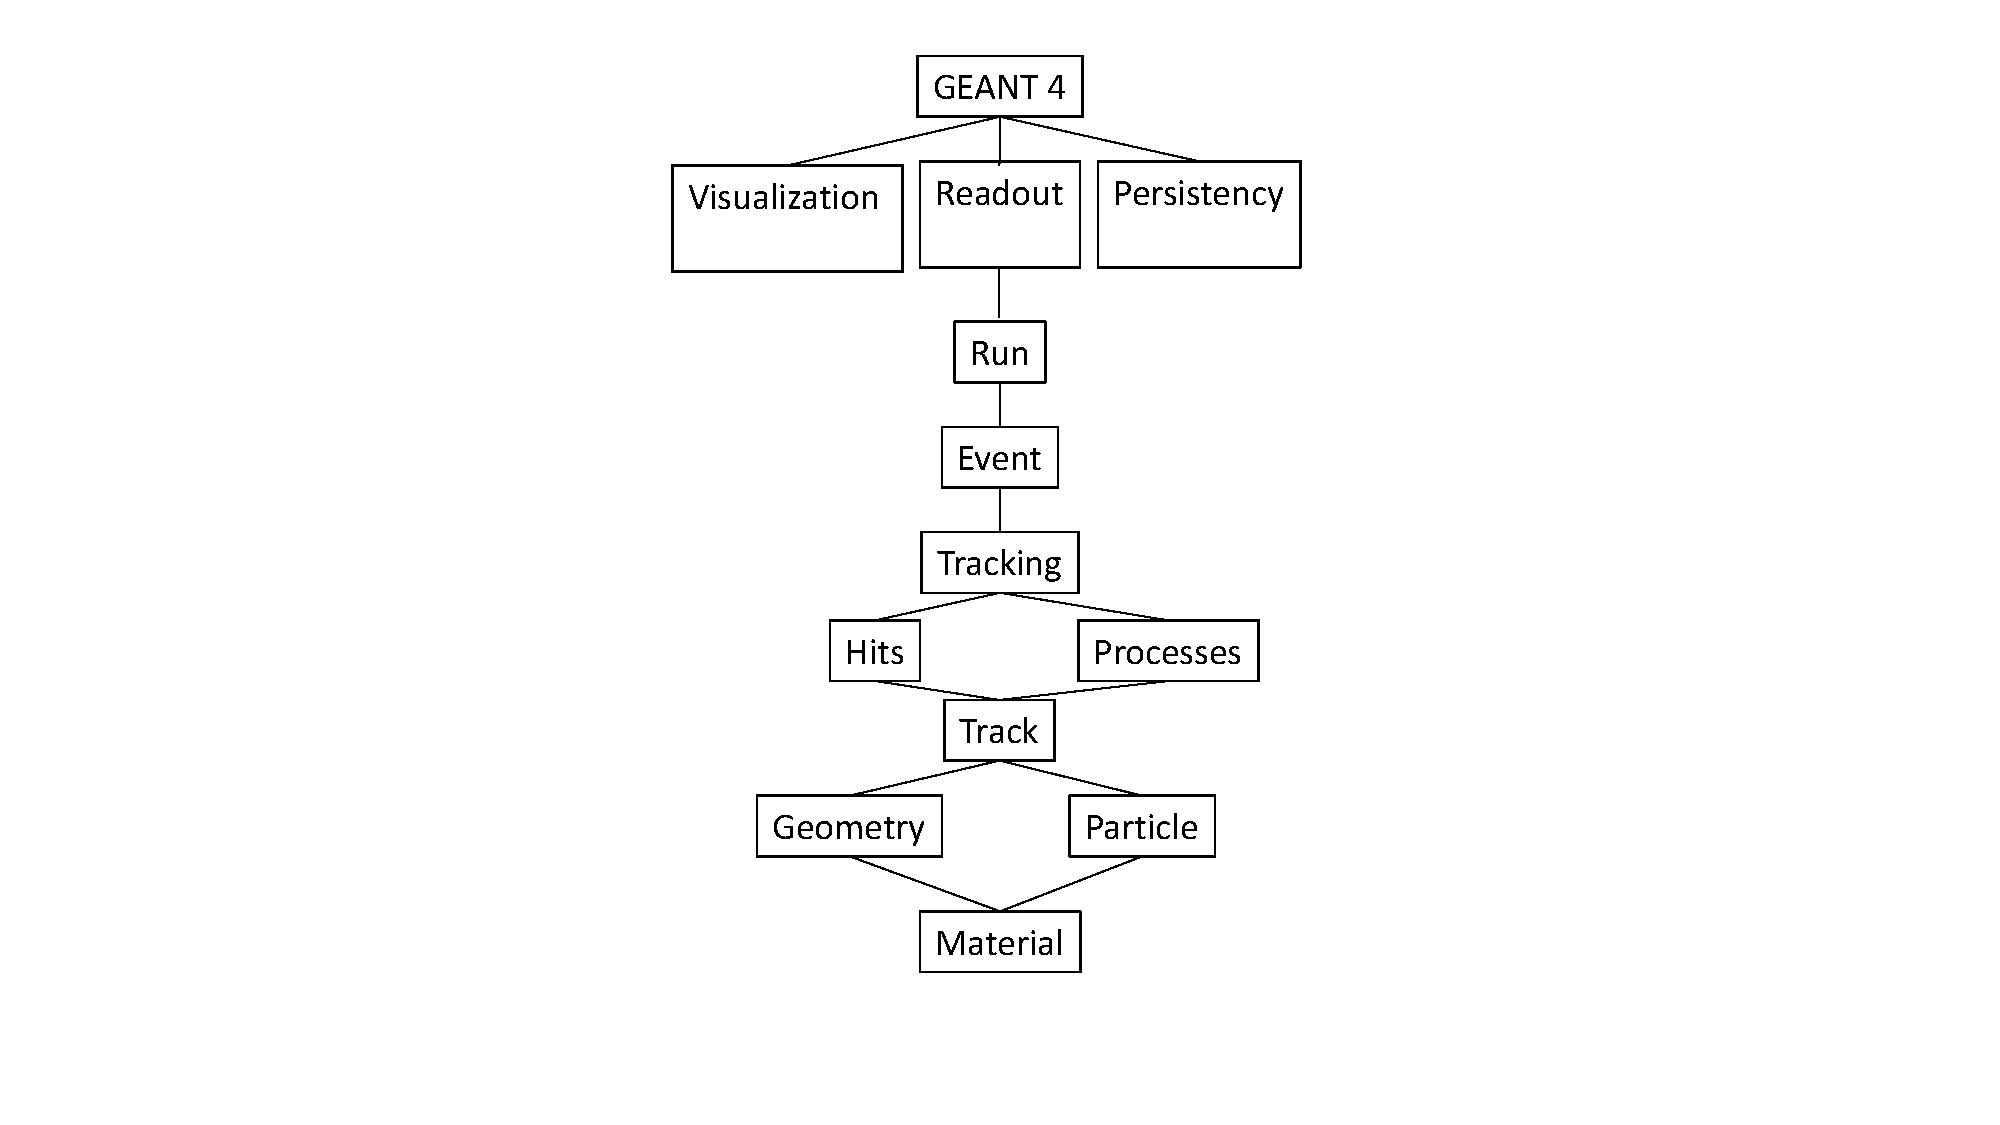
\includegraphics[width=1.7\textwidth]{figures/chapter_3/GEANT4-structure/GEANT4-structure}
\caption{GEANT4 architecture, reproduced from~\citet{Pfeier:519005}. Class structure is in the vertical direction, with dependencies towards the bottom.}
\end{figure}

\section{Representing the Earths Atmosphere}

Precipitating electrons interact with the atoms and molecules which constitute the atmosphere. The MSIS-E-90 model~\citep{Picone2002} contains a representation of the main neutral constituents of the atmosphere, their density, and temperature, parameterized by altitude and geographic location. The specific implementation of the model we use in this chapter is written in C++, which makes it compatible with the GEANT4 framework, and is available at \url{https://www.brodo.de/space/nrlmsise/index.html}. This implementation encodes the same data as the original FORTRAN version. Figure~\ref{msis_eval} shows the evaluation of this model as a function of altitude for a specific location on Earth. 

The altitude profiles of Figure~\ref{msis_eval} must be discretized and encoded as a GEANT4 geometry. This is where approximations must be made to keep the model simple enough to be computationally tractable. Each particle interaction in a GEANT4 simulation takes time to calculate and store, but additionally, an ``interaction'' occurs at the end of each particle track. The particle tracks end when a particle reaches a sufficiently low energy, but also when it crosses a physical boundary in the simulation, which exist between the faces of the simulation geometry. It is therefore critical to keep the complexity of the geometry as simple as possible. We choose to define a rectangular, Euclidean world, with vertical slices at discrete points representing the atmosphere as a function of altitude. The vertical extent of each slice is chosen to be 1 kilometer, since the major constituents of the atmosphere change density only a small amount on that scale. The horizontal extent of the simulation is set to an arbitrary large number, which for practical purposes can be taken as infinity. This ensures that particle tracks will not terminate by leaving the simulated world through the side boundaries. The model atmosphere is represented to a height of 500 kilometers above ground, beyond which the relevant particle interactions with the atmosphere very rarely occur. 

Each slice of atmosphere in the GEANT4 model is treated as a ``sensitive detector'', which is an abstraction that permits quantities such as energy deposition, entry angle, and the creation of secondary radiation to be recorded as they occur in the simulation. 
    
\begin{figure}[p]
\label{msis_eval}
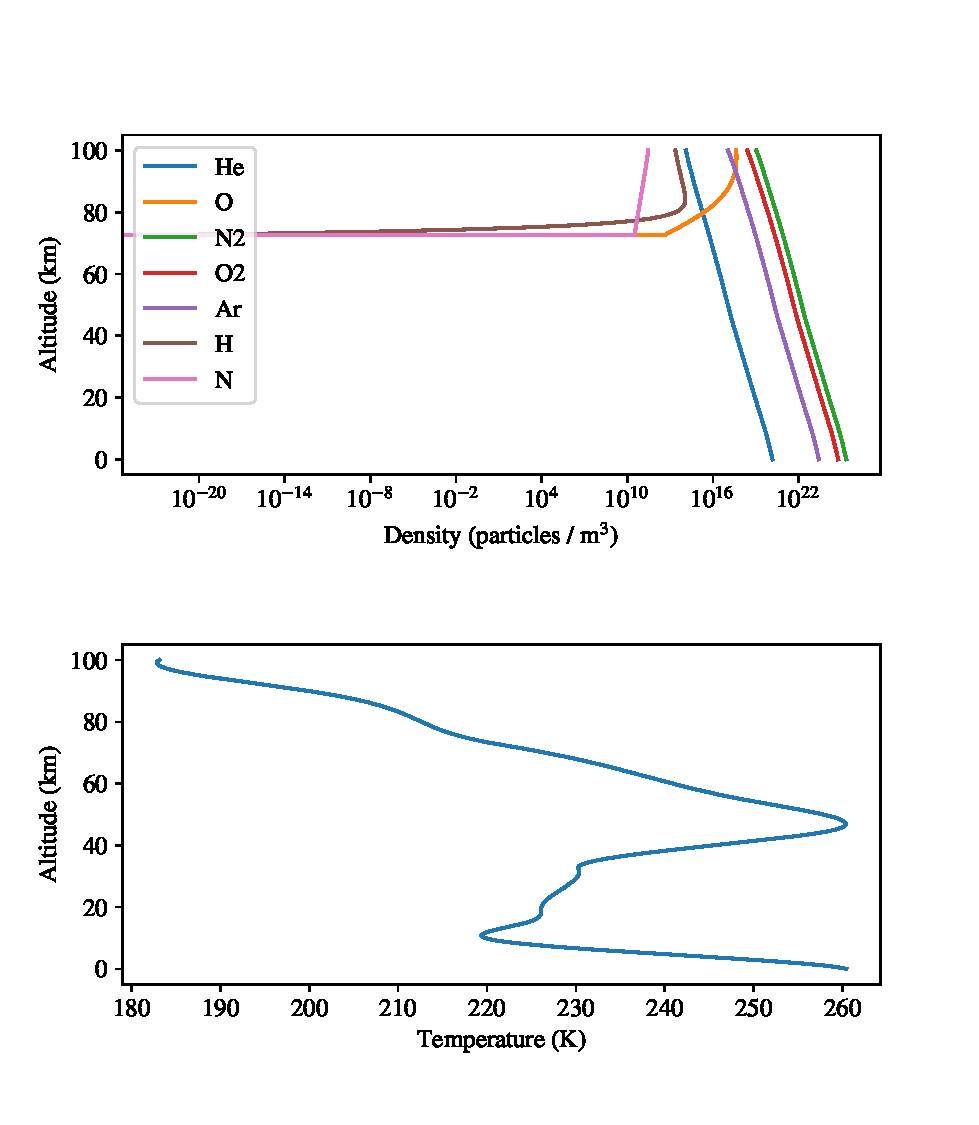
\includegraphics[width=1.0\textwidth]{figures/chapter_3/msis_eval/msis_eval}
\caption{Evaluation of key MSIS model parameters as a function of altitude. Particularly important for the GEANT4 simulation are the density profiles of each atmospheric constituent (top).}
\end{figure}

A GEANT4 volume is constructed using a stack of three abstractions. First, a G4VSolid is created, representing the shape and dimensions. The G4VSolid can be created from either a small set of geometry primitives (cylinders, boxes, and spheres), or it can be imported from an arbitrary mesh of points. The next component is called a G4LogicalVolume. This abstraction holds a reference to a G4Material, which defines the physical substance that the volume is composed of. The G4Material has the density, temperature, and molecular and atomic components of the volume material specified. The G4LogicalVolume also contains flags which control whether it is a G4SensitiveDetector, or a passive component of the simulation, through which particles are simulated but which does not return data. Finally, a G4PhysicalVolume is created which wraps the rest of the stack into one reference to one object. This object is then placed in the simulation during the initialization routine. 

\section{GEANT4 Physics and Simulation Construction}

Once the physical properties of the GEANT4 are fully specified, a selection of possible interactions between particles is chosen. There are many GEANT4 physics packages available, which are applicable over different energy ranges and for different types of particles. For this project, I chose the standard electromagnetic physics package~\citep{Burkhardt2004}. This package represents interactions between electrons, photons, and atomic nuclei from energies ranging from MeV down to keV. Effects that occur primarily below a single keV, are not represented~\citep{Guatelli2004}. Single keV photons and electrons do not travel far in the relevant parts of the atmosphere, and are quickly stopped by the materials surrounding the X-ray instrument. 

The input to the atmospheric simulation is specified by electron distributions in incident angle, and energy. Each of these are specified in GEANT4 macro files, which are text files that are used to script GEANT4 applications, and are used to avoid the need to load all the relevant data and inputs at compile time. Topside electron energy and angle distributions can be specified through a list of values, and there are also pre-built functions for the most common forms. For the Green's function approach used for this task, the input energies are a single value which is swept over the relevant energy range (100 keV to 5 MeV). 

Which angular distribution to use is not obvious, since it depends on the injection process responsible for causing the electron precipitation, the local magnetic field, and possibly other parameters. A Green's function approach here would be complicated, and the resulting simulation would need to span discrete representations of at least two dimensions. It is more practical to fix the angular distribution for a given simulation, and apply a Green's function approach only over the relevant energies. Only the electron energy spectrum can be retrieved unambiguously from the secondary Bremsstrahlung radiation~\citep{Brown2006}. This indicates that the effect of the angular distribution is small. I chose an isotropic distribution when creating this model.

The inputs to the GEANT4 simulation are then the precipitating electron distribution and total flux. The angular distribution and the model of the atmosphere are fixed. The outputs from the GEANT4 simulation are the distributions, in both angle and energy, of the produced X-ray fluxes, along with the total number of X-ray photons in the selected vertical slice of atmosphere. To obtain statistical results from the model, it is run for a large, arbitrary number of precipitating electrons. The results are represented in units per incident electron flux. The production of secondary radiation happens less at lower energies, so the chosen incident flux increases towards this limit. Because of this, the most expensive part of the simulation happens when evaluating the effect of low energy (less than 100 keV) precipitating electrons. Figure~\ref{geant4_io_schematic} shows the inputs and outputs of the GEANT4 simulation schematically. 

\begin{figure}[p]
\label{geant4_io_schematic}
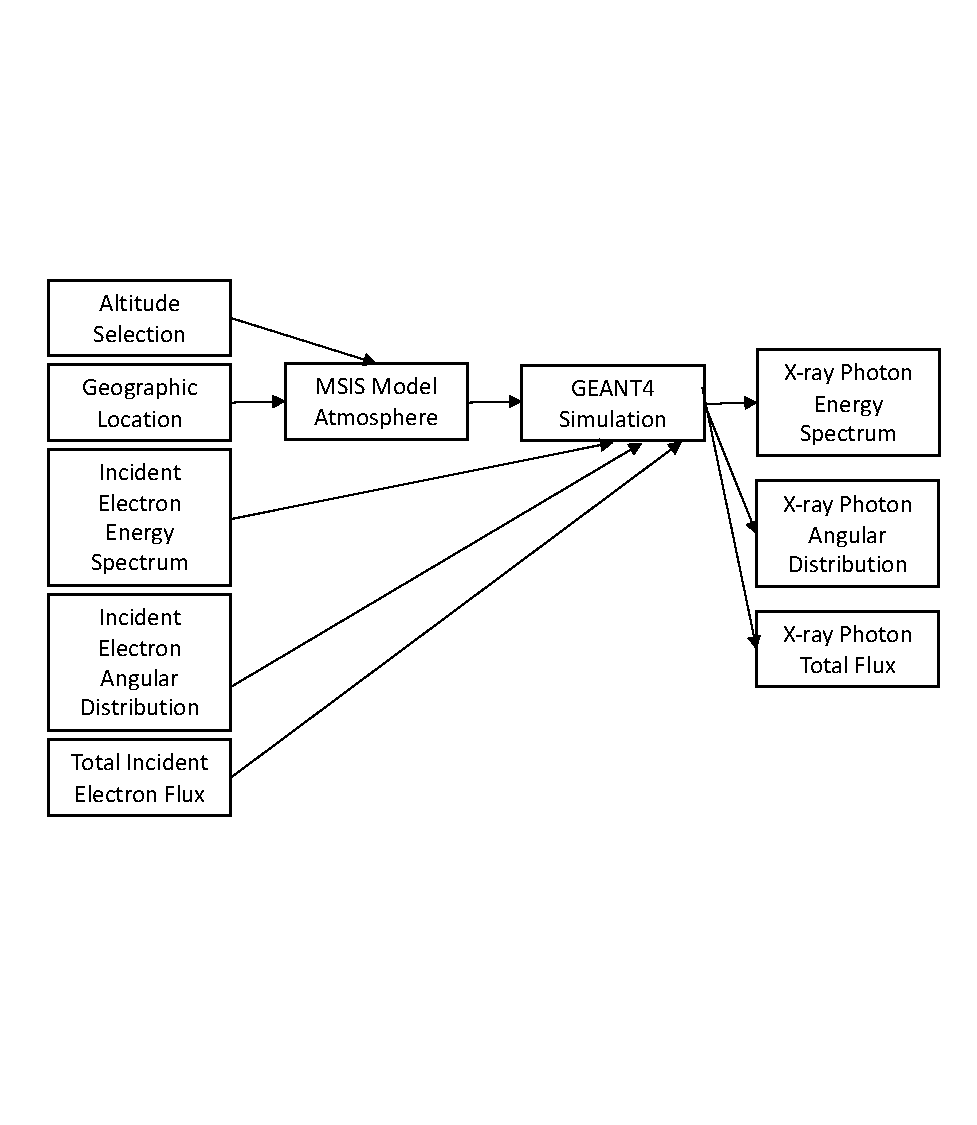
\includegraphics[width=1.0\textwidth]{figures/chapter_3/geant4_io_schematic/geant4_io_schematic}
\caption{Schematic diagram of information flow for a single GEANT4 simulation of energetic electron precipitation and the resulting X-ray radiation}
\end{figure}

The diagram in Figure~\ref{geant4_io_schematic} is the flow of information for a single GEANT4 simulation run. Since we are applying a Green's function approach, this process needs to be repeated across different monoenergetic electron beams. When this is completed, the responses to arbitrary precipitating electron distributions can then be represented as a linear combination of the recorded monoenergetic responses, without requiring further simulation runs for a fixed sample altitude and electron angular distribution. The workflow for applying the resulting data is shown in Figure~\ref{geant4_how_to_use}.

\begin{figure}[p]
\label{geant4_how_to_use}
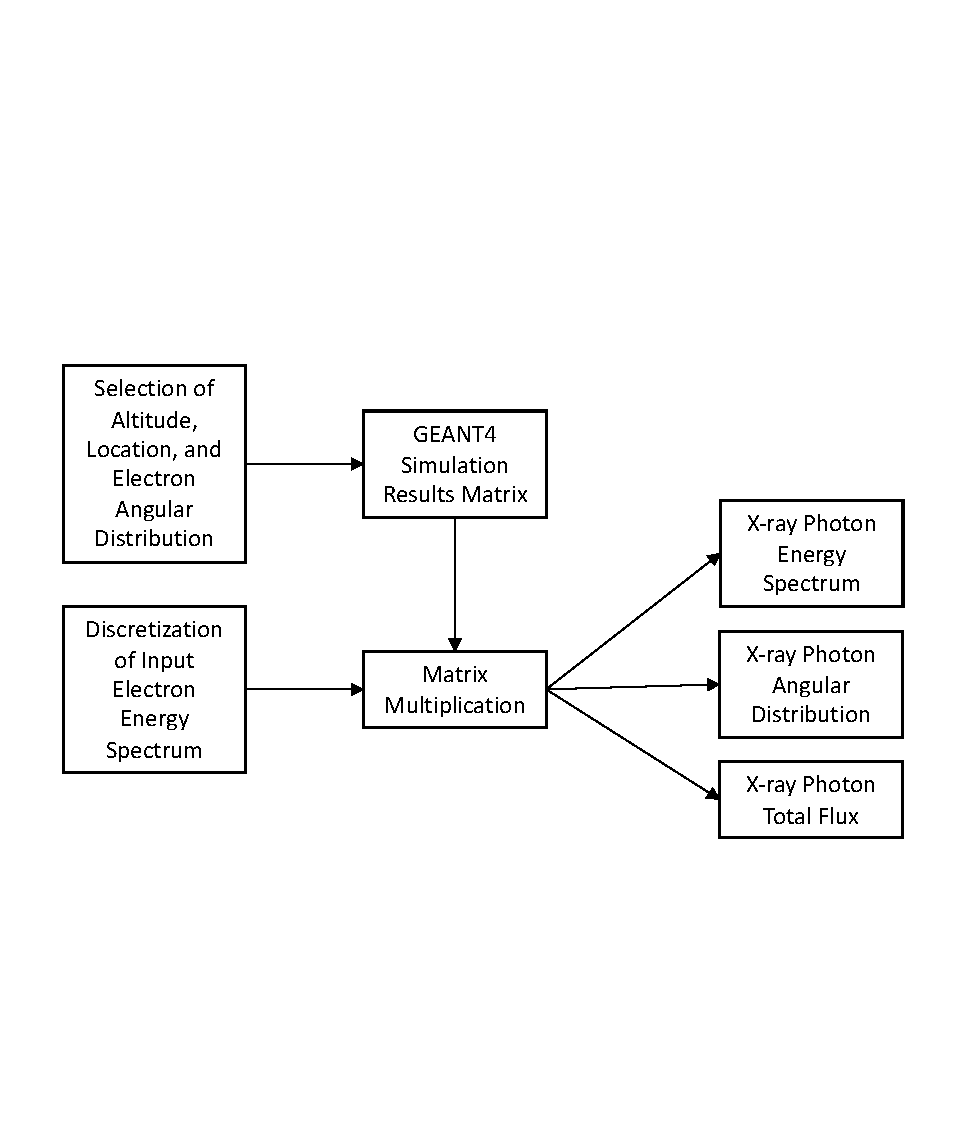
\includegraphics[width=1.0\textwidth]{figures/chapter_3/geant4_how_to_use/geant4_how_to_use}
\caption{Schematic diagram of information flow for a single GEANT4 simulation of energetic electron precipitation and the resulting X-ray radiation}
\end{figure}

The simulation of all the GEANT4 runs required is computationally expensive. Using the University of Calgary ARC computer cluster, each run was scripted to be run across the required electron energy ranges, and across unidirectional, omnidirectional, and cosine angular distributions. The simulation ranges were then evaluated again over altitudes from 30 to 34 kilometers above ground, which correspond to where viable balloon measurements of the X-ray photons can take place. In total, several weeks of computation across over 100 CPU cores were required. Once this was completed, the results were aggregated and stored in plain text files. While the computation was expensive, the results are compact, and are stored in less than one gigabyte of data.
\section{Validation of Results}

 As stated at the beginning of this chapter, the simulation problem is not new. We are reproducing the work of others so that it may be run over the parameter space we need, especially when attempting to solve the inverse problem. The first published results which we can compare to are by~\citet{Rees1963}. This author presents a semi-empirical form for the results, with a high degree of normalization to the properties of the atmosphere. The work done by~\cite{Berger1972}, on the other hand, is presented in numerical tables in physical units that are close to the output of the GEANT4 simulation. This makes them a good target for comparison to our work. 

The NASA BARREL (Balloon Array for Radiation-belt Relativistic Electron Losses) project has made their modelling work on this problem available through the SPEDAS software package~\citep{Angelopoulos2019}. The BARREL project will be discussed in Chapter~4. For now, we will only use their atmospheric simulation as a comparison to our own work. It is distributed in a format comparable to that used by~\cite{Berger1972}, and can be shown in the same parameter space. Figure~\ref{barrel_berger_spedas_comparison_34} show the expected X-ray flux, in normalized units, for isotropic incident electron beams at varying energies. The output of my model agrees with the published results in terms of the produced X-ray flux and the shape of the resulting distribution. 

\begin{figure}[p]
\label{barrel_berger_spedas_comparison_34}
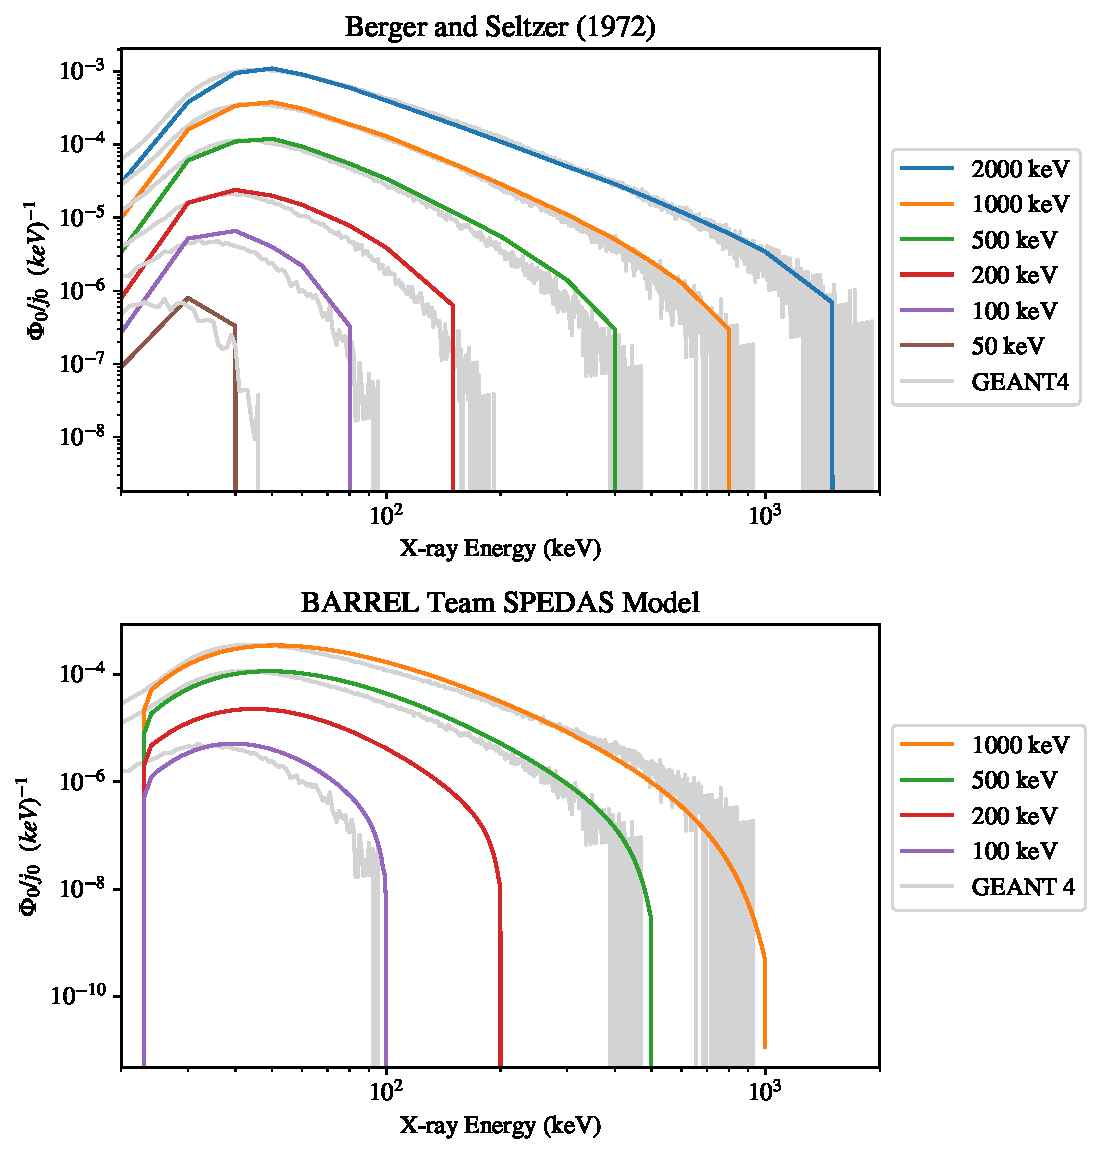
\includegraphics[width=\textwidth]{figures/chapter_3/barrel_berger_spedas_comparison/barrel_berger_spedas_comparison_alt_40km_3}
\caption{Expected X-ray flux as a function of energy at a sample altitude of 34 kilometers using data from GEATN4 simulations, ~\cite{Berger1972}, and the BARREL SPEDAS model.}
\end{figure}

\section{Problem Separability}

The distributions of photons of a given polar angle and kinetic energy are outputs from the simulation. We will show that the polar angle distribution does not depend on the energy of the precipitating electrons. This allows the results of the simulation to be expressed through their impulse responses in energy only, which is a large simplification. Figure~\ref{photon_angle_independence} shows the polar angle distribution for X-ray photons created by monoenergetic beams of precipitating electrons. Once the total photon counts are expressed in the same units, there is no significant difference in the resulting distributions.

We further show that the photon distributions in kinetic energy do not depend on the angular distribution of the precipitating electrons. This result was originally found by~\citet{Rees1963}, and implies that experiments can not recover the angular distribution of the parent electron spectrum. For the attempt at the recovery of the parent electron spectrum in the following chapter, this is useful, since this represents a degenerate dimension of the inverse problem that can be ignored. Figure~\ref{electron_angle_independence} shows GEANT4 simulations of the X-ray energy distributions caused by precipitating beams of electrons following unidirectional (downward), and isotropic angle distributions. The distributions are the same at low energies (< 200 keV), and .

\begin{figure}[p]
\label{photon_angle_independence}
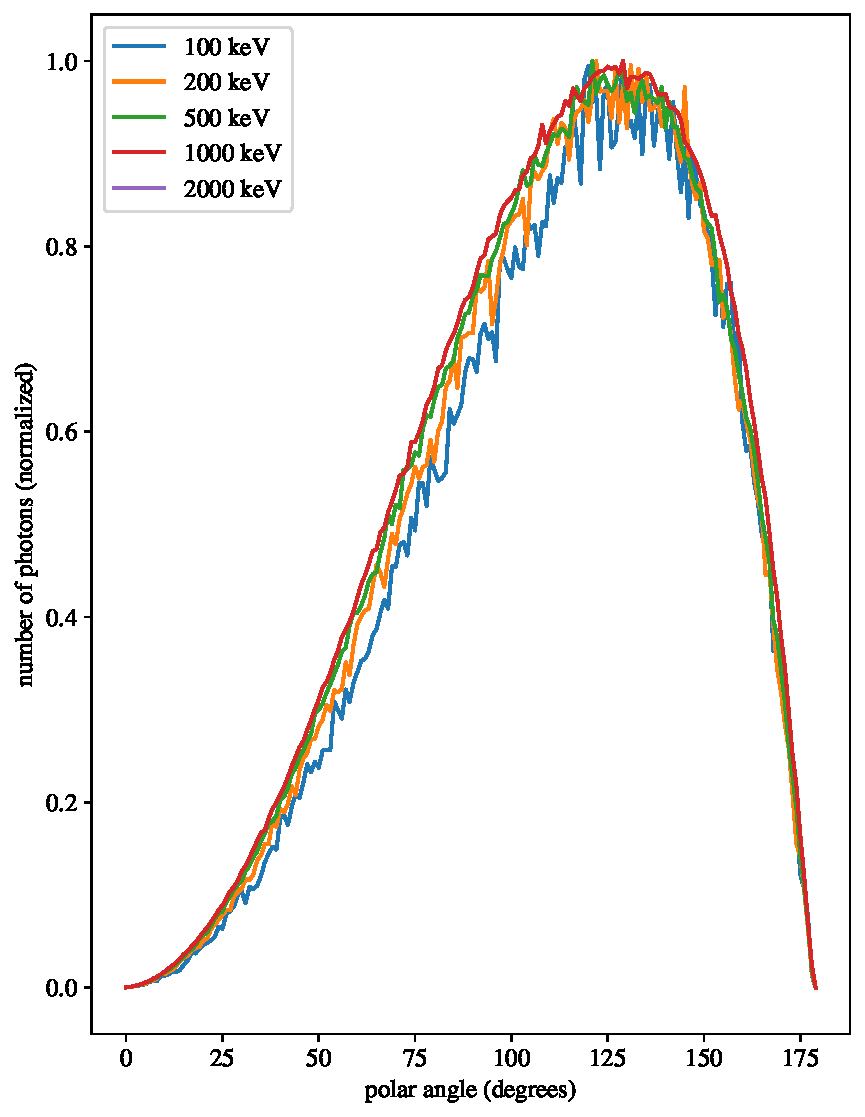
\includegraphics[width=\textwidth]{figures/chapter_3/photon_angle_independence/photon_angle_independence}
\caption{Polar angle of X-ray photon population at 34 kilometer altitude, as produced by precipitating electrons at different fixed energies. Units are normalized to account for the higher number of photons produced with greater beam energies.}
\end{figure}

\begin{figure}[p]
\label{electron_angle_independence}
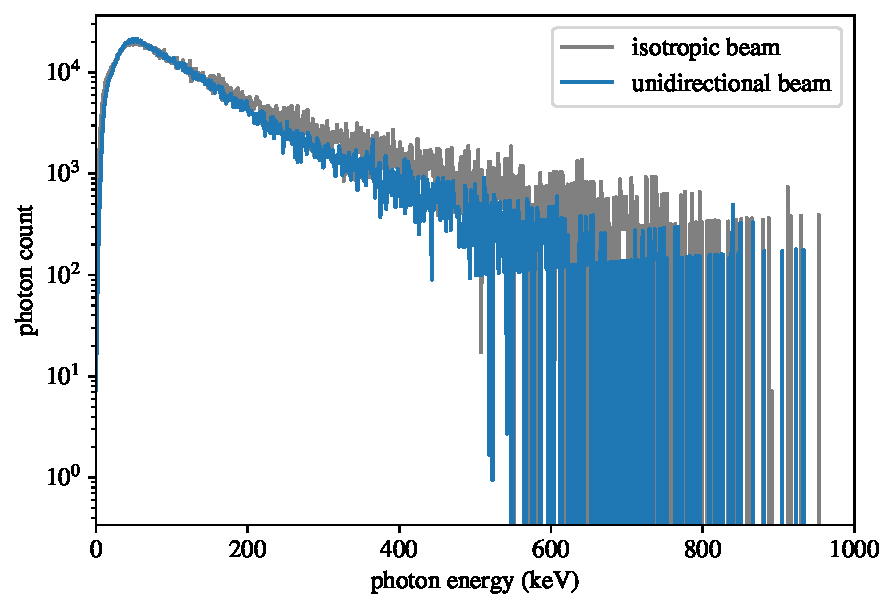
\includegraphics[width=\textwidth]{figures/chapter_3/electron_angle_independence/electron_angle_independence}
\caption{Photon energy distribution for 1 MeV incident electron beams having isotropic and unidirectional angular distributions.}
\end{figure}

The final simplification for the simulation problem comes from the parameterization of the detector response. So far we have focused on the creation and validation of the atmospheric model, which gives the angle and energy spectra of the X-ray photons which exist at the detector altitude. The detector output when it is exposed to this population will be a function of this population, and must be modelled through further simulation. The general operating principles and design of the scintillation detectors used in this experiment were described in the previous chapter. For the detector simulation, a GEANT4 model of the geometry is constructed (Figure~\ref{detector_geant4_model}.) 

\begin{figure}[p]
\label{detector_geant4_model}
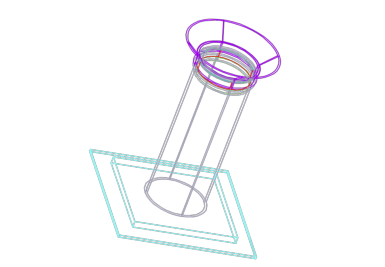
\includegraphics[width=\textwidth]{figures/chapter_3/detector_geant4_model/detector_geant4_model}
\caption{GEANT4 representation of the detector geometry. The lower plexiglass mount is shown in cyan, the aluminum body in grey, and the led collimator in purple. The height of the complete unit is approximately 30 cm.}
\end{figure}

We examine how the detector geometry selects a population from the X-ray angular distribution. In the detector simulations, an isotropic source of X-ray photons at a fixed energy are created. We run two simulations independently: the first has the entire detector geometry, with its construction materials, enabled. The material corresponding to the sodium iodide crystal, however, is set to a vacuum. This is done to measure the population of photons that reach the crystal, rather than the dynamics of the energy deposition events that happen inside of it. The second simulation is the same, except that the detector materials are set to a vacuum as well as the sodium iodide detector. This provides a baseline which we compare against the first simulation. The distribution of photons which enter the detector geometry will be subset to those recorded when the detector materials are set to a vacuum. Figure~\ref{population_inside_detector} shows the results these two simulations. The lead collimator assembly at the top of the detector has limited the field of view. Some backscatter from the detector materials can also be seen in the first simulation. 

\begin{figure}[p]
\label{population_inside_detector}
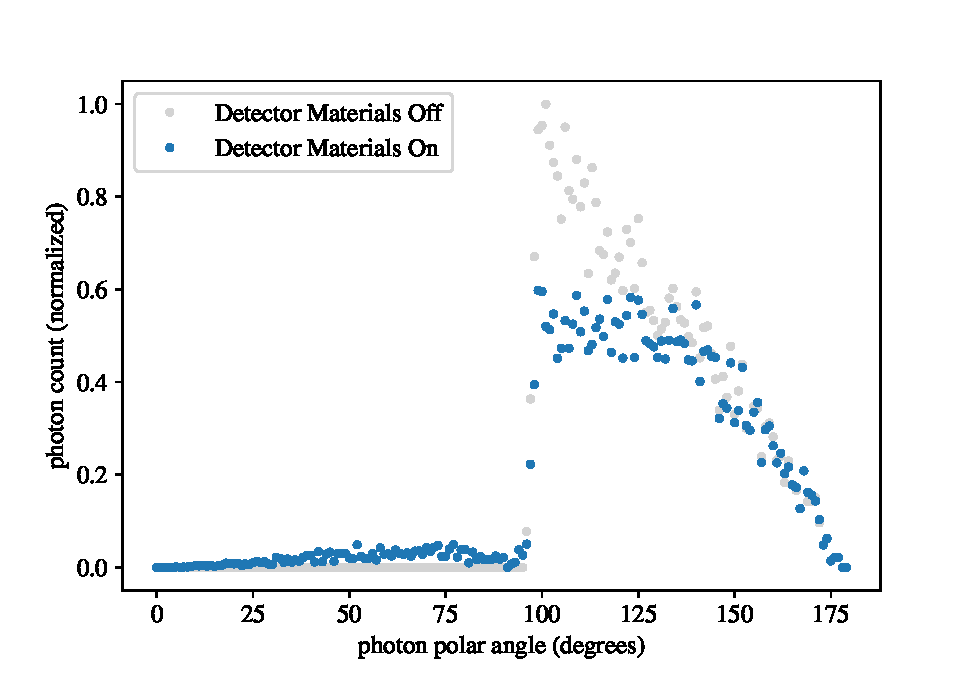
\includegraphics[width=\textwidth]{figures/chapter_3/population_inside_detector/population_inside_detector}
\caption{}
\end{figure}

The atmospheric simulation showed that the angle distribution of the X-ray photons does not significantly depend on either the angular distribution of precipitating electrons or their energy distribution. Figure~\ref{population_inside_detector} indicates that the effect of the lead collimator of the detector is essentially to limit the angle from which photons may enter the sodium iodide crystal. Together, this means that the angular portion of the complete problem from electron precipitation, to the creation of x-rays, and finally, to detection, can be largely treated as trivial. To a good approximation, and at the relevant energies (100 keV to 2 MeV), a constant scalar which accounts for the detector field of view can be used to map recorded counts to physical units.

The behaviour of the sodium iodide crystal itself to the absorption of X-ray photons is important and can also be answered through simulation. For this, the detector geometry is fully enabled in the simulation, including the sodium iodide crystal. Rather than the distributions of photon energies and angles within the crystal volume, energy deposition events will be recoded. The energy deposition events correspond to the flashes of light which are amplified by the photomultiplier tube and recorded by the detector electronics. Figure~\ref{detector_energy_response} shows histograms of the energy deposition events for a set of monochromatic photon beams. The responses can be described by delta functions at the corresponding photon energies, with interactions at lower energies which become more complex as the beam energy increases. The main interaction in this energy range is the single deposition of all the photon energy at once, which is why the peaks are easily detectable. 

\begin{figure}[p]
\label{detector_energy_response}
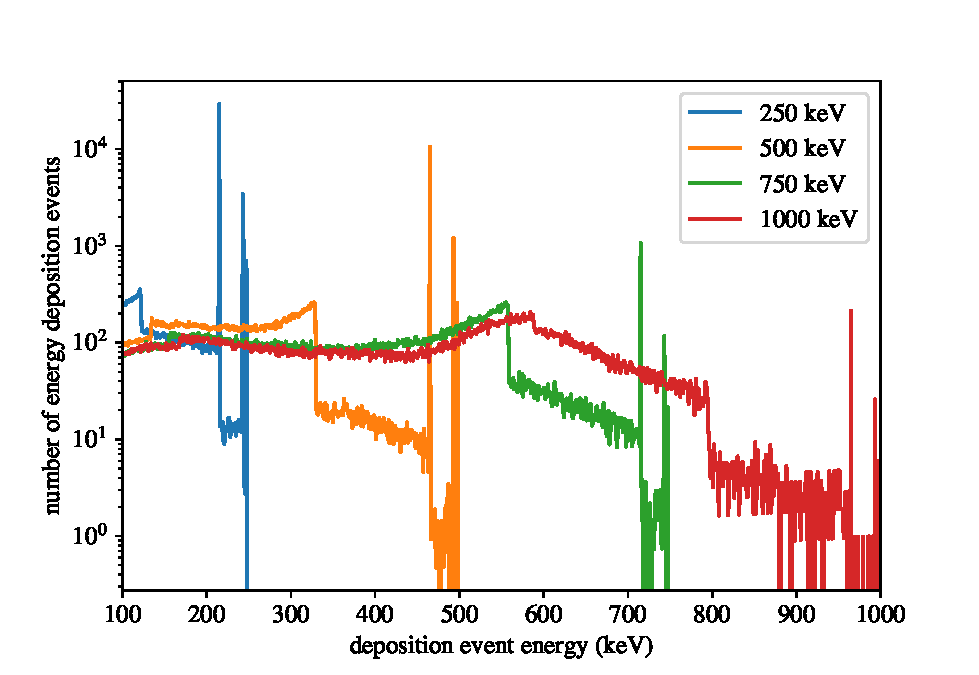
\includegraphics[width=\textwidth]{figures/chapter_3/detector_energy_response/detector_energy_response}
\caption{Energy deposition events inside the detector crystal for beams of monochromatic photons at different set energies. }
\end{figure}


 





